\documentclass[final,t]{beamer}
\mode<presentation>
  {
    \usetheme{CambridgeUS}
    \usecolortheme{seahorse}
  }

\usepackage[orientation=landscape,size=a1,scale=1,debug]{beamerposter}
\usepackage{lipsum} % for dummy text
\usepackage{graphicx}
\usepackage{tabularx}
\usepackage[export]{adjustbox}
%\usepackage{vcell}
\setbeamertemplate{caption}[numbered]

\title[]{\huge PSD Parameterization to support ice retrievals from multiple
instrument observations}
\author[]{\large Mircea Grecu$^{1}$, Gerald Heymsfield$^{2}$, John Yorks$^{2}$, and Andrew Heymsfield$^3$}
\institute[]{\Large (1) Morgan State University,  (2) NASA GSFC, and (3) NCAR}
\date{}

\begin{document}

\begin{frame}
\maketitle
\begin{columns}[]
  \begin{column}{.32\linewidth}

\begin{block}{Motivation}
\begin{itemize}
\item
  Current and future air- and space-borne observing systems feature
  instruments with different sensitivities and subject to attenuation at
  different ranges.
\item
  From the scientific perspective, physically consistent ice property
  estimates are desirable irrespective of the instruments used in their
  derivation.
\item Such estimates may be derived through the development of consistent "a priori"
probability distributions.
\end{itemize}
\end{block}

\begin{block}{Approach}
\begin{itemize}
\item  Use "in-situ" Particle Size Distributions (PSDs) to simulate lidar and radar observations at X-, Ku-,Ka- and W- band.
\item  Develop kNN methodology to estimate ice properties from combination of observations.
\item Test methodology using cross-validation.
\item Evaluate using independent estimates.
\end{itemize}
\end{block}

\begin{table}[ht]
%\caption{A table arranging  images}
\centering
\begin{tabular}{cc}
\includegraphics[scale=0.85]{IMPACTS_Nw.png}&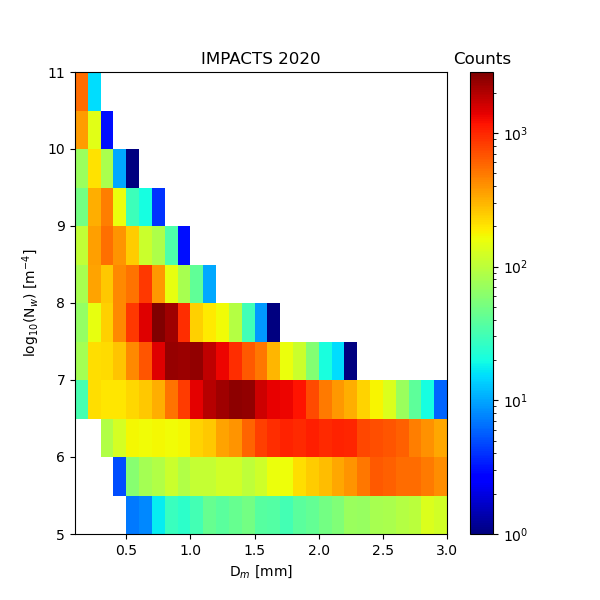
\includegraphics[scale=0.85]{IMPACTS_Nw_dm.png}\\

%\multicolumn {2}{c} 
\end{tabular}
\end{table}
\centerline{The $N_w$ distribution as a function of temperature and the $N_w-D_m$ joint
distribution}

\centerline{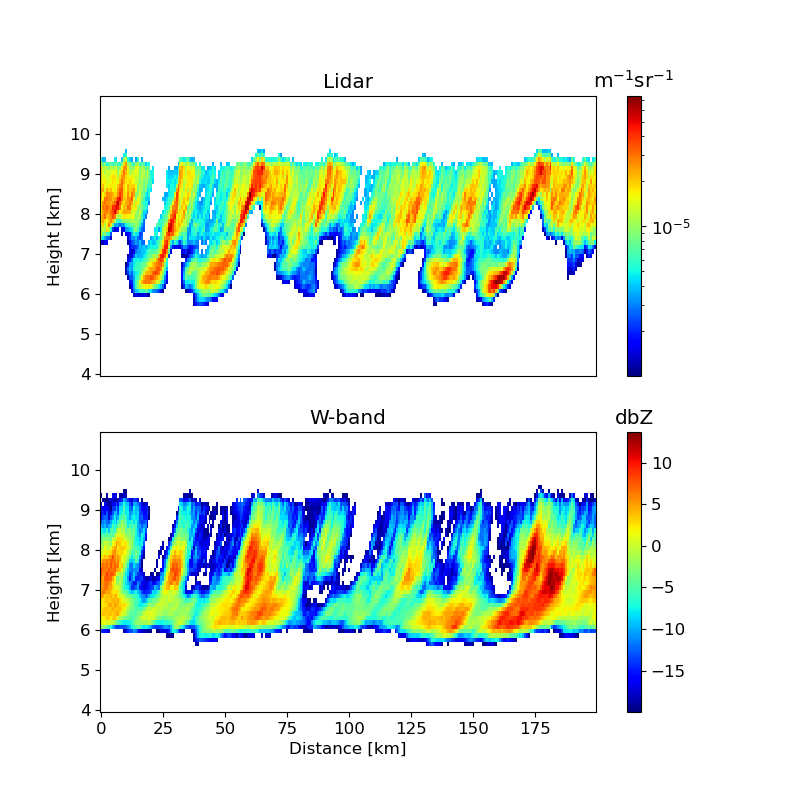
\includegraphics[scale=0.95]{radarAndLidar_slice.png}}
\centerline{Simulated lidar backscatter and radar reflectivitiy.}

\begin{itemize}
\item
In the combined radar lidar region, the lidar backscatter and the integrated backscatter can be used
as constraints for the kNN methodology.
\item
In the region of single frequency radar observations, temperature can be directly used as a parameter,
over via $N_w$ in "normalized relationships" e.g. $IWC=N_w^{1-b}aZ_w^b$.
\end{itemize}
\end{column}


 %%%%%%%%%%%%%%%%%%%%%%%%%%%%%%%%%%%%%%%%%%%%%%%%%%%%%%%%%%%


  \begin{column}{.32\linewidth}

  \begin{block}{Cross-Validation Results}
  \begin{itemize}
   \item
   For evaluation in the simulation space, the database of observed PSDs and calculated reflectivities is randomly split in two.
   \item
   Half of the database is used for training, while the other is used for evaluation.
   \item
   Results are shown below.  Errors are likely to be caused by ambiguities in the database, rather than
   methodology.
  \end{itemize}
  \end{block}
\begin{table}[ht]
%\caption{A table arranging  images}
\centering
\begin{tabular}{cc}
\includegraphics[scale=1]{dmValidation.png}&\includegraphics[scale=1]{iwcValidation.png}\\
\end{tabular}
\end{table}

\begin{block}{Direct Validation Results}
\begin{itemize}
\item
 "In-situ" and retrieved IWCs for two cases from the 2020 campaign are shown below.
 \end{itemize}
\end{block}
  \centerline{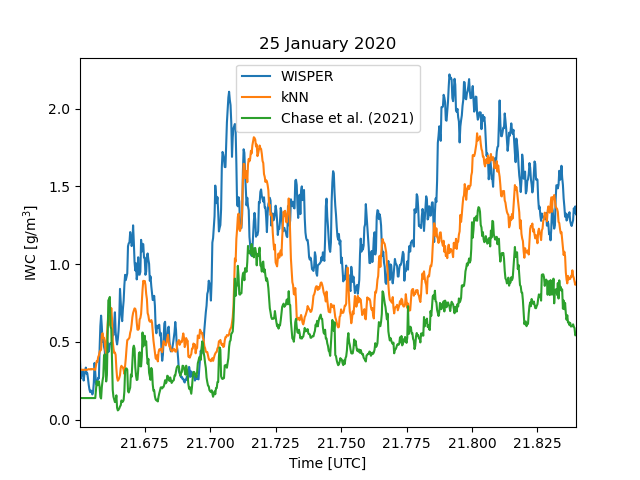
\includegraphics[scale=1.25]{jan25_2020.png}}
  
  \centerline{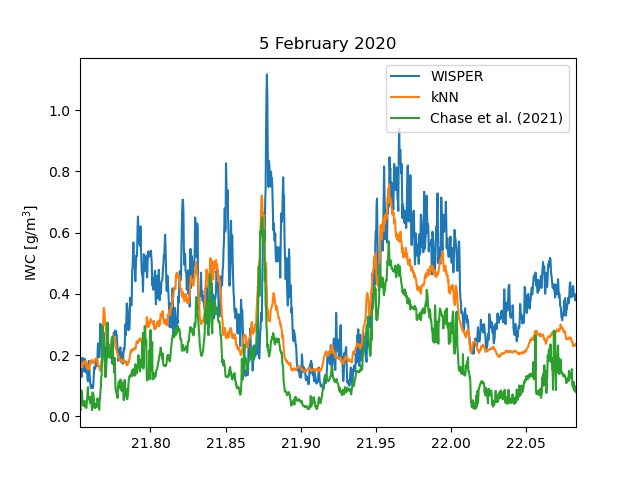
\includegraphics[scale=1.25]{feb05_2020_2.png}}
  
%\begin{table}[ht]
%\caption{A table arranging  images}
%\centering
%\begin{tabular}{cc}
%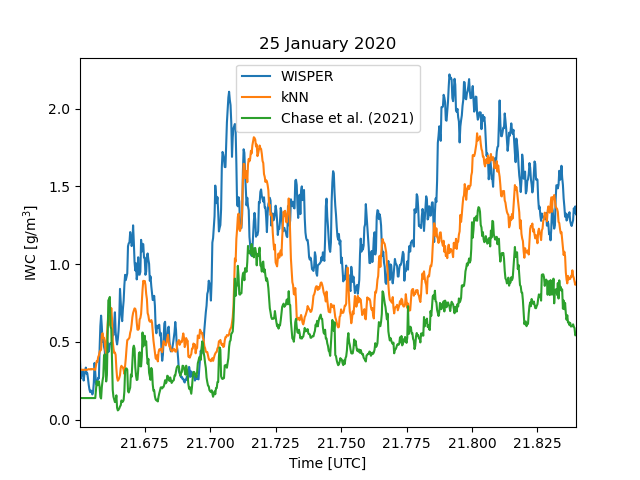
\includegraphics[scale=0.75]{jan25_2020.png}&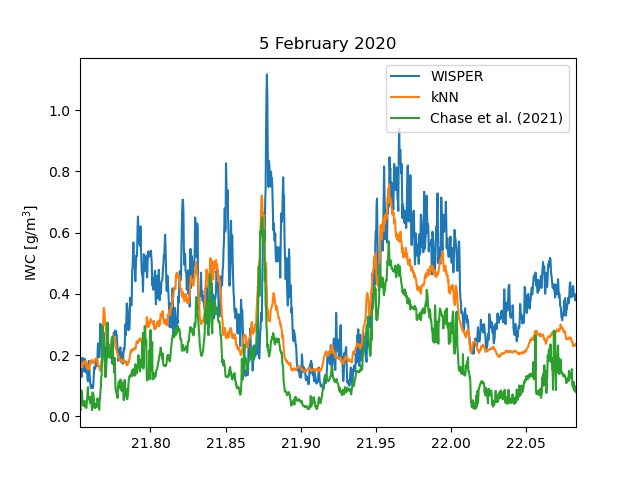
\includegraphics[scale=0.75]{feb05_2020_2.png}\\
%\end{tabular}
%\end{table}
\end{column}


  %%%%%%%%%%%%%%%%%%%%%%%%%%%%%%%%%%%%%%%%%%%%%%%%%%%%%%%%%%%

  \begin{column}{.32\linewidth}

  \begin{block}{Comparisons between retrievals}
   Single frequency (W-band) and multiple but low sensitivity (Z$_{Ku}$ and Z$_{Ka}>$10 dBZ) retrievals
   are compared.
  \end{block}
  
   \centerline{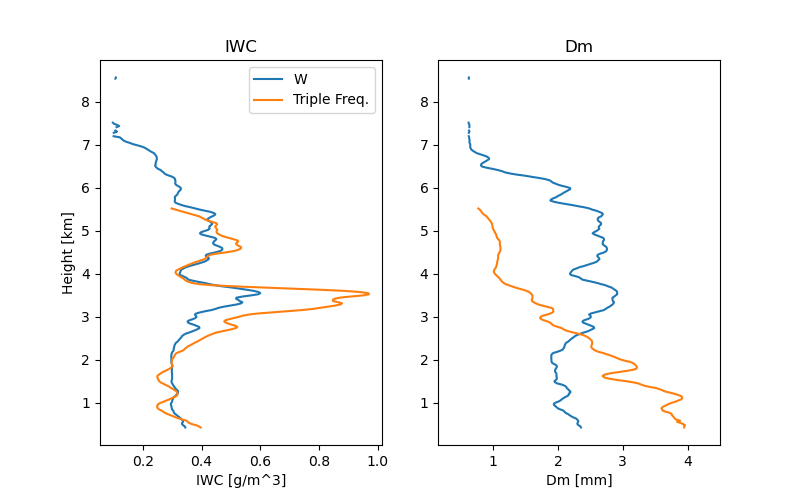
\includegraphics[scale=1.25,valign=t]{retrievedProfs.png}}
   
   
\begin{table}[]
%\caption{A table arranging  images}
%\centering
\begin{tabular}{p{13cm}p{13cm}}
\begin{itemize}
\item
Discrepancies appear to be larger in terms of $D_m$ than in terms of IWC.
\item
At the top of the echo, multiple frequency IWC tends to be larger than the W-band estimate
because the DFR(Ku,Ka) is close 0.
\item
Near the surface single frequency IWC tends to be larger than the multiple frequency estimate.
Attenuation at W-band may exacerbate differences.
\item
A parameterization of D$_m$ as a function of temperature, e.g 
$D_m=2.68\cdot 10^{-4} \cdot {T_c}^2+2.67\cdot 10^{-2} \cdot {T_c}+8.62\cdot 10^{-1}$ seems to better mitigate
uncertainties than a Nw parameterization.
\item
The D$_m=f(T_c)$ parameterization may be combined with a $D_m=f(DFR)$ parameterization to further mitigate uncertainties.
$D_m=0.00228\cdot DFR^3 -0.0336 \cdot DFR^2+0.3486\cdot DFR+0.2668$
\end{itemize}
 &
 \includegraphics[scale=0.85,valign=t]{retCmp.png}\\
 \end{tabular}
 
 
 \end{table}
  
  \begin{block}{Concluding remarks}
   \begin{itemize}
   \item
   The cross-validation and the direct comparisons suggest good retrieval performance.
   \item
   In the cross-validation evaluation, triple frequency retrievals are more accurate than dual and single frequency retrievals.
   \item
   However, in practice, triple frequency retrievals (or at least the most complex formulations) may not be as robust as simpler formulation.
   \item 
   A $D_m$ driven approach is likely to be the best option in transitioning from  single to multiple 
   frequency retrievals.
   \end{itemize}
 \end{block}
 
  \end{column}
  
 
  \end{columns}

\end{frame}

\end{document}
